%%% Fiktivní kapitola s ukázkami sazby

\chapter{Analýza problému a jeho řešení}

V této kapitole je detailně popsán problém a způsoby jeho navrženého a současného řešení.

\section{Úvod}

Spoje které zajišťují hromadnou dopravu jezdí podle jízdních řádů, které definují jejich trasu. Trasa se udává sekvencí projíždících zastávek, časy příjezdu a odjezdu do, resp. z těchto zastávek a vzdáleností zastávek od výchozího bodu spoje. Tyto zastávky jsou zpravidla jediné refenční body u kterých je možno zjistit skutečné zpoždění, nebo předjetí (dále uvažováno jako zpoždění se zápornou hodnotou). Dále jsou součástí jízdních řádů také velice detailní nákresy tras každého spoje, formou lomené čáry definovanou posloupností souřadnic, kde každý bod je doplněn o jeho vzdálenost od výchozího bodu spoje.

\bigbreak

Délka trasy mezi dvěma refernčními body nezříka dosahuje i několika desítek kilometrů\footnote{Podle dat pro spoje jedoucí v 20. 2. 2020 je medián vzdálesnotí mezi zastávkama, mezi kterýma projede alesponˇ jeden spoj denně 943 m. Průjezdů mezi zatávkami ve vzdálenosti více než 10 kilometrů je 784, přiřičemž průjezdů mezi zastávkami ve vzdálenosti alesponˇ 2 km je přibližně 15000}. Na těchto úsecích mohou vznikat mimořáné události, které se dají predikovat jen s těží. Nicméně ve většině případů je průběh jízdy ovlivněn pouze obvyklým provozem v dané denní době.

Detailní rozbor počtu průjezdů mezi zastávkami v daných vzdálenostech je vidět na grafu \ref{fig:stop_distances_result}. Kde průjezdem se myslí každý jednotlivý průjezd vozidla mezi danou dvojcí zastávek v daný den. Data jsou platná pro spoje jedoucí v 20. 2. 2020.

\begin{figure}
	\centering
  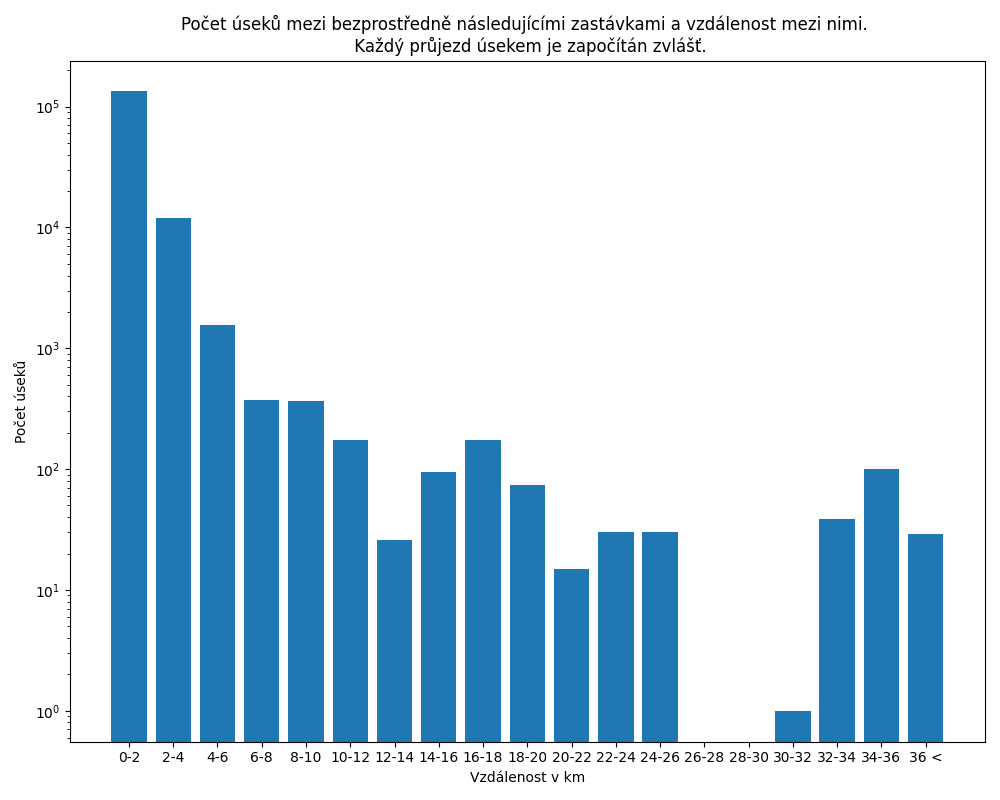
\includegraphics[width=0.6\linewidth]{../img/stop_distances_plot_2020-02-20.png}
  \caption{Graf počtu úseků mezi následujícími zastávkami a vzdálenotí mezi nimi.}
  \label{fig:stop_distances_result}
\end{figure}

\section{Popis problému odhadu zpoždění}

Řešený problém se týká případu, kdy vozidlo projíždí mezi dvěma referenčními body a tato trasa má části, ve kterých vozidlo jede různou rychlostí. Např. vozidlo při vyjíždění z města jede mnohem pomaleji než při jízdě mezi městy. Takových úseků, na kterých se rychlost jízdy liší může být na trase více a nedají se všechny jednoduše detekovat.

\bigbreak

Tato Práce tedy modeluje profily jízd mezi referenčními body. A na základě toho zpřesnit odhad zpoždění. Tento odhad by měl být mnohem přesnější než současné odhady, které odpovídají tomu, že vozidlo jede konstantní rychlostí po celou dobu jízdy. Nebo je takové možné brát jako aktuální zpoždění spoje poslední změřené zpoždění při průjezdu nějak7ch referenčním bodem (zastávkou, nebo např. pro tramvaje se používají návěstidla).

\bigbreak

Přidaná hodnota je tedy v tom, že Práce navrhne takové modely, které nebudou penezalizovat zvyšováním zpožděním za pomalou jízdu v úsecích, které se pomaleji projždějí vždy. A také naopak zvýhodnˇovat snížením zpožděním za rychlou jízdu v úsecích, které se projíždějí rychle. Pokud bychom se tedy podívali na změny zpoždění na trase mezi dvěma referečními body, v ideálním případně by měli být nulové.

\bigbreak

Pro řešení toho typu spoždění stačí navrhnout systém na odhat zpoždění v půběhu jízdy mezi referenčními body z historikých dat jízd.

\bigbreak

Pro vyloučení všech pochybností je hodno uvést, že se naše Práce nesnaží předpovědět zpoždění, které spoj může nabrat vzhledem k dosavadnímu průběhu trasy. Tedy např. nijak nezohlednˇuje to, že spoj právě stojí v mimořádné koloně a dalo by se tedy předpokládat, že zpoždění bude rychle růst i v následujících minutách. Ale naopak Práce se snaží odhadnou zpoždění v danném bodě na trase vzhledem k obvyklému profilu jízdy. Tedy např. pokud by výše uvažavaná kolona byla pravidelná Práce ji zohlední ve statistických modelech.


\subsection{Příklad nelineárního profilu trasy}

Celé ilustrováno na příkladě jízd mezi dvěma zastávkama K letišti a ZLičín, kde je nelineární profil jízdy vidět velice dobře. Jedná se totiž o trasu přesně odpovídající popisu problému.

\bigbreak

Popsané rozdíly v rychlosti a nelineární profil trasy je patrný na grafu \ref{fig:k_letisti_to_zlicin_3d}. Za povšimnutí táké stojí viditelné spomalení průjezdů v ranní špičce, 7--9 hodina ráno.

\begin{figure}
  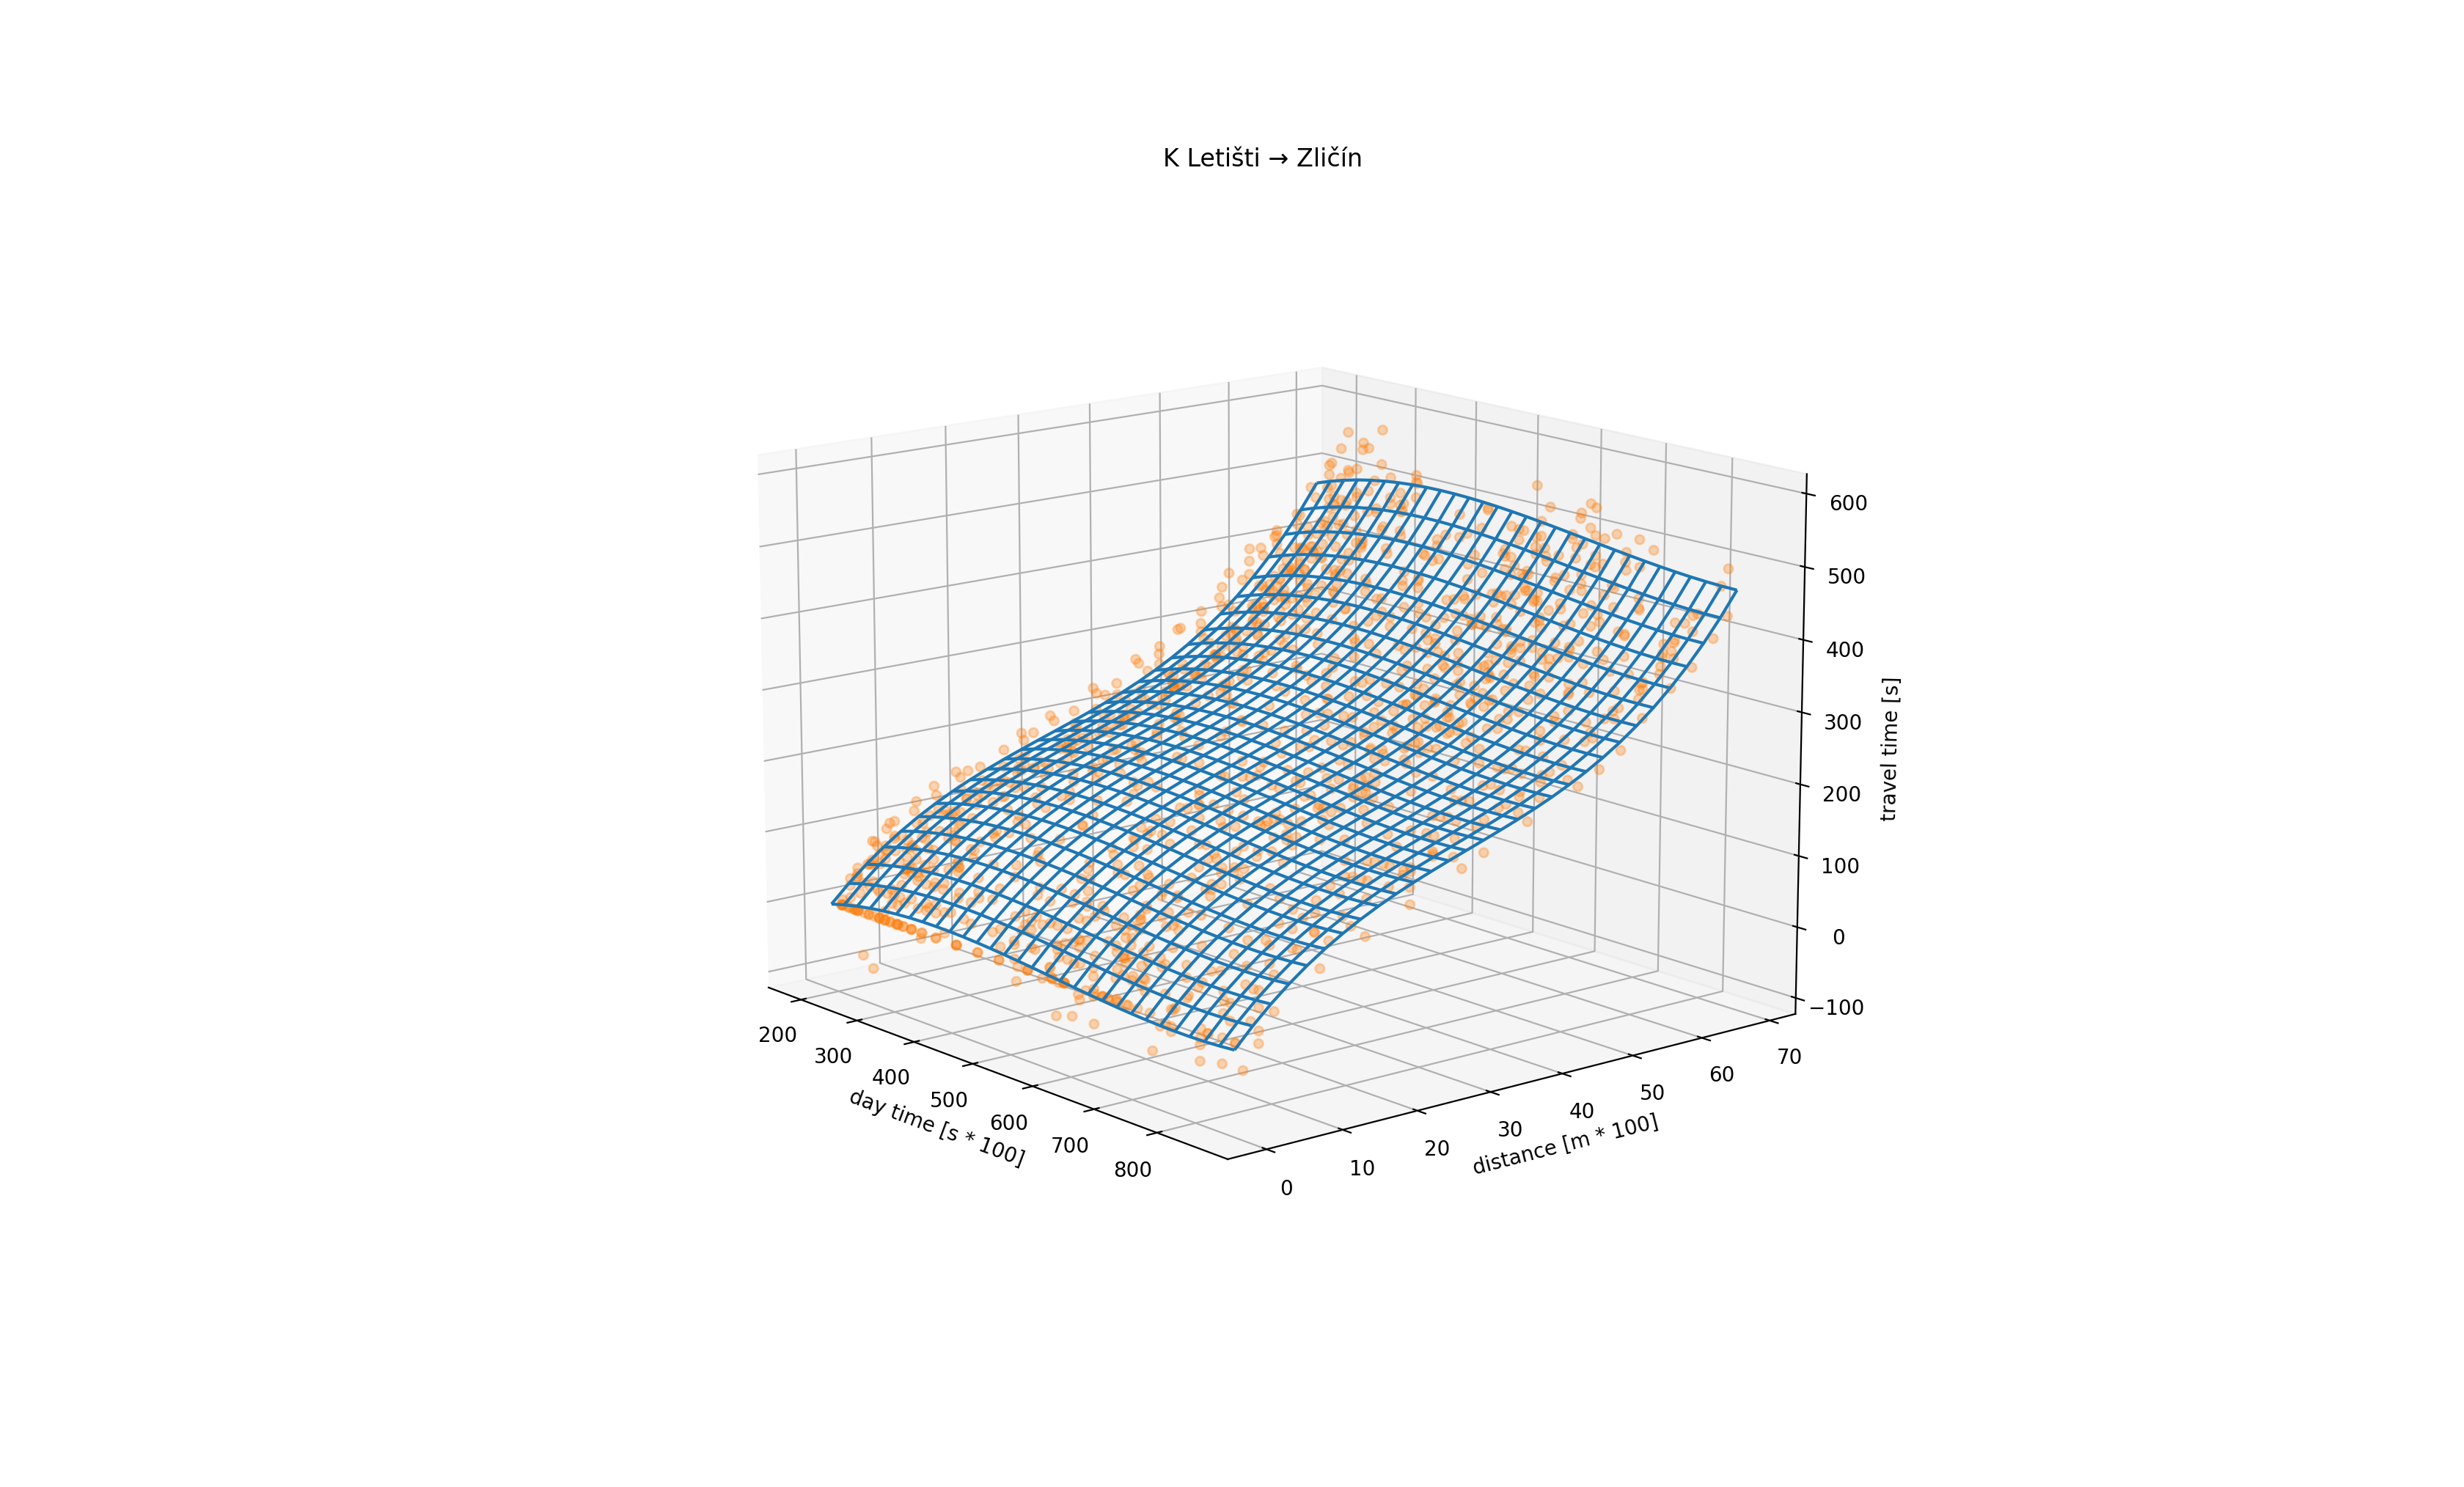
\includegraphics[width=\linewidth]{../img/k_letisti_to_zlicin_3d.png}
  \caption{Modrá plocha značí vymodelovaný profil trasy. Oražové body jsou jednotlivé vzorky polohy vozidel. Data pro graf jsou ze dnů 20.--21. 2. 2020}
  \label{fig:k_letisti_to_zlicin_3d}
\end{figure}

\bigbreak

Na obrázku \ref{fig:k_letisti_to_zlicin_map} je pro bližší představu popsané trasy vidět trasa spoje vykreslená do mapy.

\begin{figure}
	\centering
  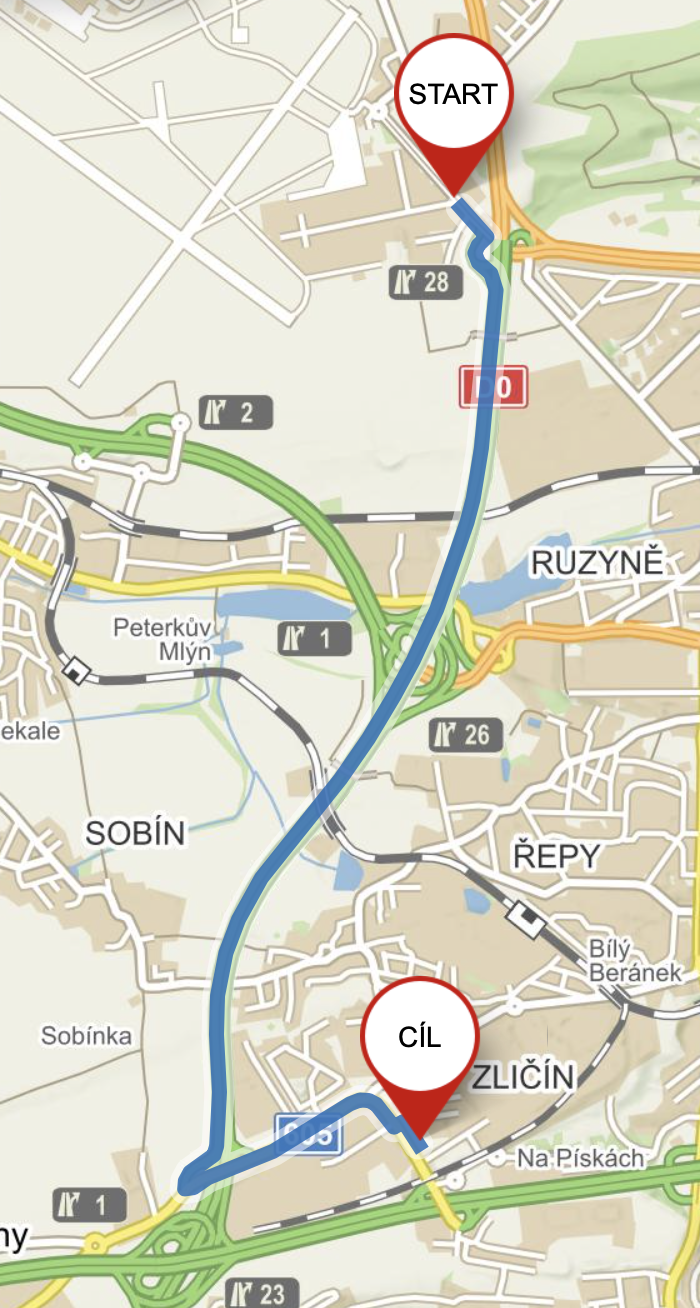
\includegraphics[width=0.3\linewidth]{../img/k_letisti_to_zlicin_map.png}
  \caption{Trasa mezi zastávkama K Letišti a Zličín. Zdroj: mapy.cz}
  \label{fig:k_letisti_to_zlicin_map}
\end{figure}

\subsubsection{Rozbor trasy}

Celá tato trasa má necelých 7 km a její průjezd spojem VHD trvá 10 minut. Prvních 600 metrů je vedeno po obecní komunikaci, přes křižovatku a nájezd na Pražský okruh. Průměrná rychlost vozidel byla 35 km/h\footnote{Počítáno podle vozidel, které poslaly polohu v 600m (resp. 4.9km, resp. 6.6km pro další údaje o rychlosti) vzdálenosti od zastávky. Počet záznamů o poloze vozidel se v různých vzdálenostech liší.}.

\bigbreak

Dále trasa pokračuje přes Pražský okruh rovně až do vzdálenosti 4.9 km od zastávky K Letišti, kde začíná nájezd na ulici Na Radost. Dá se předpokládat, že vozidla se na komunikaci vyšší třídy pohybují rychleji což dokazuje, že na tomto úseku trasy se průměrná rychlost vozidel zvýšila na 63 km/h.

\bigbreak

Poslední úsek se tedy skládá z výjezdu z Pražského okruhu, průjezdu křižovatkou, jízdy po obecní komunikaci a vjezdu do stanice Zličín. Délka úseku je 2 km. Průměrná rychlost za celou trasu se na tomto úseku snížila na 55 km/h.

\subsection{Současná řešení}

Takový algoritmus na odhat aktuálního zpoždění mezi dvěma referenčními body již exituje a je součástí Datové Platformy -- Golemio, ze kterého se čerpají data pro tuto práci. (Detailní popis dat uveden v kapitole ~\ref{chapter:TODO later}.) Nicméně nezohledňuje variabilitu profilu trasy. Tento algoritmus totiž nahlíží na postup vozidla na trase jako na lineární funkci vůči času. Je ovšem zřejmé, že rychlost vozidel není konstantní, neboli doba jízdy není linárně závislá na ujeté vzdálenosti.

\bigbreak

Proto je potřeba tento odhad zpřesnit, což je cílem naší práce.
